\chapter{Introducci\'on}
\label{cap:intro}

\section{Antecedentes y motivaci\'on}
\label{intro:motivacion}

Investigadores del Departamento de Física de la Universidad de Santiago de Chile pertenecientes al Centro para el Desarrollo de la Nanociencia y la Nanotecnología (CEDENNA) trabajan en la simulación de los efectos del campo magnético en los átomos de distintos objetos, tomando en cuenta su forma, su material y su distribución atómica, entre otras características.

La simulación consiste en ejecutar eun programa computacional que implementa el Método Monte Carlo Cadenas de Markov (MCMC, \emph{Monte Carlo Markov Chain}) sobre una grilla tridimensional de átomos. Uno de los grandes problemas de los usuarios de este software es que el proceso previo y posterior a la simulación es ``manual''. Para definir el objeto a simular deben hacer un dibujo en Microsoft Paint\textregistered, el cual es analizado por un \emph{script} de Matlab\textregistered\ que debe ser modificado para reflejar las características del objeto específico que se quiere simular. Para generar imágenes para, por ejemplo, una publicación, también deben ejecutar ciertos \emph{scripts}, sin embargo esto es aún más complicado, ya que deben hacer ensayo y error hasta conseguir que la imagen sea representativa del resultado, puesto que muchas veces tienen errores de visualización que no reflejan el estado real del sistema. Estos dos sub-procesos hacen que el proceso de simulación sea tedioso, quitando mucho tiempo que podría ser usado en analizar los resultados.

Es aquí donde la informática puede contribuir, creando aplicaciones que mejoren estos procesos, que valoricen el tiempo de los científicos. Por consiguiente esta es una oportunidad única de ayudar a la obtención de conocimientos que permitan entender el entorno y de mejorar los procesos que permiten avanzar como sociedad hacia la comprensión del universo.


\section{Descripci\'on del problema}
\label{intro:problema}

El proceso actual de diseño de estructuras atómicas a simular y su visualización ha sido creado por distintos investigadores que han sido parte del CEDENNA, los cuales en general solo tienen conocimientos básicos de diseño y desarrollo de software, esto ha llevado a que este proceso se base mayoritariamente en \emph{scripts} de \emph{MatLab}, los que deben ser modificados y ejecutados manualmente para ir obteniendo los resultados deseados, esto resulta en la posibilidad de que los usuarios introduzcan errores fácilmente, los que pueden ser muy difíciles de detectar debido a la mala calidad de las pre-visualizaciones que se logran. Debido a la naturaleza de esta solución se requiere de un prolongado periodo de tiempo para poder generar datos para las simulaciones.

Una vez ejecutada la simulación es necesario poder visualizar los resultados de esta, para lo cual también se basan en \emph{scripts} de \emph{MatLab}, los que después de un largo proceso, debido a las distintas configuraciones manuales que deben hacer, genera imágenes de calidad pobre para publicaciones. Esto genera una gran pérdida de tiempo para los investigadores.

A continuación se describe con más detalle el proces actual que los investigadores realizan.


\section{Proceso actual}

\subsection{Diseño de objetos para simular}

Actualmente los científicos no tienen un proceso definido y formal de creación de objetos para simulación, ya que existen diversas soluciones implementadas a través del tiempo, desde \emph{scripts} escritos en \emph{MatLab} que fueron creados especialmente para diseñar un objeto en específico hasta unos \emph{scripts} más genéricos, pero igualmente engorrosos, usando como base un mapa de bits.


\subsubsection{Diseño programático de objetos}

La primera opción para diseñar objetos es de manera programática, es decir, escribiendo un \emph{script} que defina todas las partículas de un objeto y sus vecindades. Para alguien con experiencia en esta área puede ser relativamente sencillo diseñar algunos objetos regulares, como por ejemplo un cilindro, no obstante el proceso se complica si se quieren diseñar estructuras irregulares. Dado que la visualización del objeto diseñado es de muy baja calidad con este sistema es fácil cometer errores que eventualmente pueden invalidar los resultados de una simulación.

La figura \ref{procesoactualacript} muestra un ejemplo de la visualización de un \emph{script} de MatLab que genera un cilindro con radio $R = 60nm$ y altura $H = 20nm$ escalado a un sistema con solo 4 capas de átomos.

\begin{figure}[ht]
  \centering
  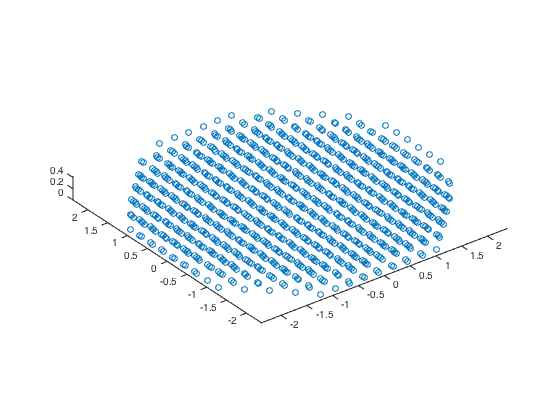
\includegraphics[scale=.6]{images/procesoActualScript}
  \caption{\em Ejemplo de imagen salida de un \emph{script} de generación de objeto}
  \label{procesoactualacript}
\end{figure}

\subsubsection{Diseño en base a mapa de bits}
\label{intro:procesoactualmapa}

Para flexibilizar el diseño de objetos y bajar la posibilidad de introducir errores en los datos de entrada se creó un sistema que permite especificar la geometría de un objeto en base a un mapa de bits construido en \emph{Microsoft Paint}. De esta forma no es necesario escribir un progama cada vez qe se cambiase la geometría del objeto, si no que basta con crear una imagen que representa la primera capa del objeto y usar el \emph{script} de \emph{MatLab} para el tipo de estructura cristalina específica que se desea definir.

\begin{figure}[ht]
  \centering
  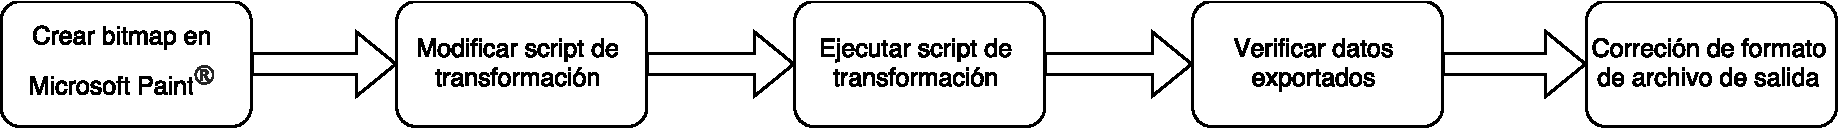
\includegraphics[scale=.5]{images/procesoActualBitmapFlujo}
  \caption{\em Flujo para creación de diseño de objetos en base a mapa de bits}
  \label{procesoActualBitmapFlujo}
\end{figure}

Como se puede ver en la figura \ref{procesoActualBitmapFlujo}, para iniciar este proceso es necesario tener un editor de imágenes que permita crear archivos .bmp, como por ejemplo Microsoft Paint\textsuperscript{\textregistered}. Con este editor se crea una imagen del tamaño y forma deseada, la cual usualmente no excede los 50px x 50px. Luego se debe pintar, con color negro, los pixeles que representen la primera capa de átomos del objeto. Estos pixeles luego serán identificados por un \emph{script} de \emph{Matlab}, como posiciones relativas de átomos del objeto.

En la figura \ref{procesoActualBitmap} siguiente imagen se muestra un ejemplo de estos mapas, usando una imagen de 10px x 10px. Esta figura solo representa la forma y posiciones relativas de los átomos y no considera el tipo de átomo ni la estructura cristalina que ellos forman.

\begin{figure}[ht]
  \centering
  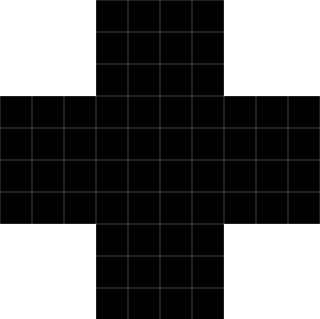
\includegraphics[scale=.6]{images/procesoActualBitmap}
  \caption{\em Mapa de bits de 10px x 10px}
  \label{procesoActualBitmap}
\end{figure}

Para introducir esta información se debe modificar otro \emph{script} de \emph{Matlab}, el cual tiene múltiples versiones según el tipo de estructura cristalina que se quiera diseñar, que agrega los parámetros físicos del objeto. Algunas de las opciones que se deben configurar antes de iniciar la ejecución son:

\begin{description}
	\item [Número de capas] \hfill \\
		Cuántas veces se repite la primera capa para formar un objeto en 3D.
	\item [Coeficiente de escalamiento] \hfill \\
		Es un coeficiente usado para dar al objeto las medidas deseadas para ejecutar la simulación.
	\item [Constante de red] \hfill \\
		Esta es la dimensión real (en nanómetros) de la arista de una celda unitaria
\end{description}

Todos estos parámetros deben ser modificados directamente en el código, y en distintas partes de este, por lo que es muy fácil cometer errores, los que por supuesto invalidan cualquier simulación hecha en base a estos.

Una vez configurado el script, este debe ser ejecutado. Se lee el mapa de bits ingresado como parámetro analizando cada uno de los pixeles, creando un arreglo binario de 2 dimensiones, donde un pixel negro es representado por un 1 y un pixel blanco es representado por un 0, lo que creará la primera capa de átomos; luego, según las configuraciones ingresadas, generará el resto de átomos buscados con sus correspondientes vecinos. El resultado es un archivo con las posiciones de los átomos y sus vecinos, además de dos imágenes que representan las distintas partículas generadas en base a los archivos de entrada. Estas imágenes no son lo suficientemente claras como para poder identificar errores en el diseño esperado, por lo que la posibilidad de equivocarse y simular con una premisa inválida es algo mucho más común que lo esperado.

La figura \ref{procesoActualMatlab1} muestra la visualización 3D del objeto de la figura \ref{procesoActualBitmap} generado con \emph{MatLab}. Como se puede apreciar esta visualización no permite distinguir claramente la forma de cruz del objeto. Solo una vista 2D, como la de la figura \ref{procesoActualMatlab2}, permite corroborar la forma adecuada.

\begin{figure}[ht]
  \centering
  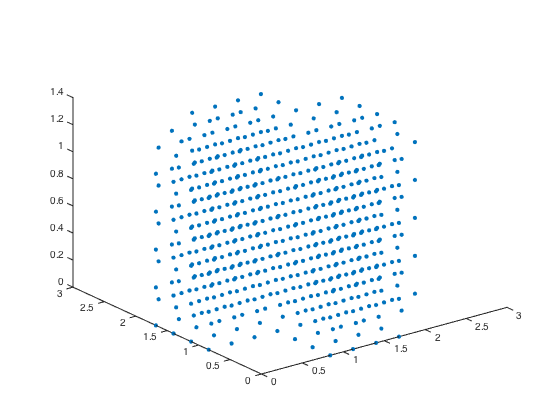
\includegraphics[scale=.6]{images/procesoActualMatlab1}
  \caption{\em Vista 3D de los átomos encontrados}
  \label{procesoActualMatlab1}
\end{figure}

\begin{figure}[ht]
  \centering
  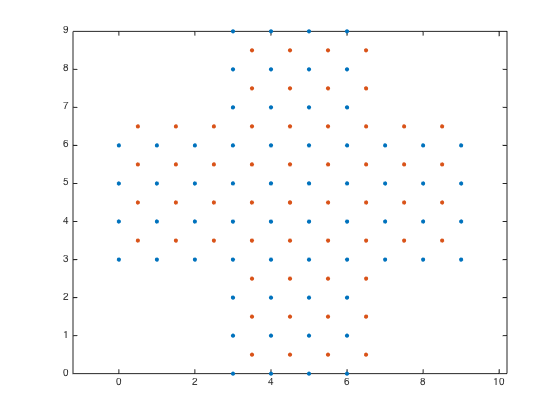
\includegraphics[scale=.6]{images/procesoActualMatlab2}
  \caption{\em Vista 2D de la primera capa de átomos}
  \label{procesoActualMatlab2}
\end{figure}

Una vez decidido que el objeto diseñado se usará para una simulación es necesario ejecutar un nuevo software, escrito en C, que se encarga de modificar el archivo de salida del script de \emph{Matlab} de tal forma de que pueda ser usado como entrada para la simulación Monte Carlo. Cabe notar que este software está compilado y no se cuenta con el código fuente de este, de tal forma que si en algún momento se necesitara modificar el formato de la entrada de la simulación este software se debería re-escribir.

La transformación consiste en modificar cada línea del archivo, con el siguiente formato:

\begin{center}
	\begin{lstlisting}
 5.4700000e+02   1.4000000e-01   1.5400000e+00   1.2600000e+00   4.0000000e+00   4.8300000e+02   4.8400000e+02   4.8700000e+02   4.8800000e+02   0.0000000e+00   0.0000000e+00   0.0000000e+00   0.0000000e+00
	\end{lstlisting}
\end{center}

\noindent
y eliminar todas las potencias, reemplazándolas, de ser posible, con números enteros. Además es necesario agregar una línea en el inicio del archivo que contiene distintos parámetros usados por el software de simulación, como el número de partículas y la constante de escalamiento.

Un ejemplo de las primeras 5 líneas de un archivo correcto sería:

\begin{center}
	\begin{lstlisting}
 104	1	8	0.00245
 1	-0.19799	-1.26	0	3	3	4	54	0	0	0	0	0
 2	0.19799	-1.26	0	3	4	5	55	0	0	0	0	0
 3	-0.39598	-1.12	0	4	1	6	7	58	0	0	0	0
 4	0	-1.12	0	6	1	2	7	8	52	59	0	0
	\end{lstlisting}
\end{center}

En la primera línea los datos necesitados son:
\label{formatoDatos}

\begin{itemize}
	\item Número de átomos descritos en el archivo
	\item $1$. Este valor no se utiliza y se mantiene por razones de compatibilidad con antiguas versiones del software de simulación
	\item Número máximo de vecinos
	\item Constante de escalamiento
\end{itemize}

Desde la segunda línea en adelante el formato es:

\begin{itemize}
	\item ID del átomo
	\item Componente $\hat{i}$ de la ubicación
	\item Componente $\hat{j}$ de la ubicación
	\item Componente $\hat{k}$ de la ubicación
	\item Cantidad de vecinos del átomo
	\item ID del vecino 1
	\item ID del vecino 2
	\item ...
	\item ID del vecino N
\end{itemize}

En caso de que un átomo tenga un número vecinos inferior al máximo posible se deben rellenar la línea con ceros, de tal forma que cada línea tenga la misma cantidad de valores.

\subsection{Visualización de resultados}

Si bien el proceso de diseño de objetos es precario, este no se compara con el de visualización y exportación de resultados, tanto en forma de imágenes como videos. Dentro de las limitaciones actuales está la imposibilidad de generar videos con colores que permitan distinguir una tercera dimensión.

Actualmente se usa la funcionalidad \emph{Quiver plot} de \emph{MatLab}, que permite dibujar rápidamente vectores en base a archivos de entrada con cierto formato, no obstante este proceso requiere de tiempo para obtener representaciones que realmente reflejen lo deseado, siendo un proceso de ensayo y error que utiliza tiempo de manera innecesaria para los científicos.


% Actualmente los investigadores deben preparar la simulación usando un \emph{script} en Matlab\textregistered, el cual analiza un archivo \emph{.bmp} creado en \emph{Microsoft Paint\textregistered}, esta imagen generalmente es pequeña, menor a 50px x 50px, y representa la primera capa del objeto (mirado desde arriba), para esto se marcan los pixeles que describen el objeto, de esta forma el mapa de \emph{bits} es binario, si un \emph{pixel} es negro se considera un 1, si es blanco se considera un 0. En este \emph{script} se describen características específicas del objeto que se quiere definir, entre ellos:
% \begin{itemize}
% 	\item Número de capas: Cuantas veces se repite la primera capa para formar un objeto en 3D.
% 	\item Distribución de los átomos (ver anexo A): Como premisa se trabaja sólo con distribuciones cúbicas de átomos, no obstante estas distribuciones tienen ciertas características específicas, por ejemplo:
% 	\begin{itemize}
% 		\item Cúbico simple (SC por \emph{Simple Cubic}): En cada vértice de una distribución cúbica se encuentra un átomo.
% 		\item Centrado en las caras (FCC por \emph{Face-centered Cubic}): Además del átomo en cada vértice de la distribución cúbica, hay un átomo en el centro de cada cara de la distribución.
% 		\item Centrado (BCC por \emph{Body-centered Cubic}):  Además del átomo en cada vértice de la distribución cúbica, hay un átomo en el centro de cada distribución.
% 	\end{itemize}
% 	\item Coeficiente de escalamiento: Es un coeficiente usado para dar al objeto las medidas deseadas para ejecutar la simulación.
% \end{itemize}

% Este proceso produce un archivo de texto plano describiendo cada uno de los átomos del objeto sobre el cuál se aplicará la simulación.

% Luego de ejecutada la simulación el software entrega múltiples archivos de texto, uno que define cada uno de los átomos con un ID y una posición en el espacio, y N archivos que definen la fuerza magnética de cada átomo en un tiempo dado. Los científicos deben seleccionar uno de estos archivos y aplicar un \emph{script} de Matlab\textregistered\ para poder visualizar el resultado.

% El proceso de exportación de imágenes para publicaciones puede tomar un día de trabajo para los científicos, ya que deben hacer ``ensayo y error'' hasta que la imagen producida refleje lo que desean. Luego deben esperar por la aprobación por parte del profesor guía, en caso de ser rechazada, deben volver a ejecutar el proceso.

% \subsection{Soluciones similares}
% Existe una herramienta que hace simulaciones similares a las que hace el grupo de científicos llamada ``Go Parallel Magnet\textregistered''. A pesar de que la simulación no es exactamente la misma, el flujo de diseño es útil para el proyecto. Sin ir más lejos los científicos basan el proceso actual en éste.

% ``Go Parallel Magnet\textregistered'' usa para el diseño un sistema de multi-capas, donde se define la capa superior del objeto y se indica la cantidad de veces que ésta se repetirá. Con estos datos se crea un objeto en 3D que luego se transforma en la estructura molecular deseada.

\section{Propósitos de la solución}
\begin{enumerate}
  \item Automatizar el proceso de diseño de configuraciones atómicas usadas para la simulación, de forma de disminuir tanto el tiempo requerido para esto como la probabilidad de introducir errores humanos, los que pueden inválidar una simulación
  \item Permitir el manejo interactivo durante el diseño de una configuración atómica mediante rotaciones, traslaciones y \emph{zoom}
  \item Exportar configuraciones atómicas que puedan ser simuladas inmediatamente, sin necesidad de transformar los datos
  \item Generar imágenes de alta calidad para publicaciones, tanto de una configuración atómica diseñada como de un estado de la simulación en un tiempo $t$
  \item Generar videos de cambios de estados de una simulación para presentación en conferencias
\end{enumerate}


\section{Alcances o limitaciones de la solución}
\begin{itemize}
	\item El software se encargará del diseño de objetos para la simulación entregando la entrada para ésta y posteriormente de la visualización de los resultados, y de la exportación de estos para publicaciones, mas no se encargará de la simulación en sí, la cual queda fuera del alcance de la solución.
	\item La aplicación estará disponible para sistema operativo MAC OS X.
	\item El diseño de objeto será por capas, es decir, se define la ``vista superior'' y la cantidad de veces que se repetirá hacia abajo.
\end{itemize}

\section{Objetivos y alcance del proyecto}
\label{intro:objetivos}

\subsection{Objetivo general}
Diseñar e implementar una aplicación para el diseño interactivo de configuraciones atómicas 3D, basado en capas, y para la visualización dinámisa y estática de la evolución de dicha configuración durante una simulación de campo magnético.

\subsection{Objetivos espec\'ificos}

Para la consecución del objetivo general, se plantean las siguientes metas intermedias para el proyecto:

\begin{enumerate}
  \item Definir los requerimientos funcionales, en base a la interiorización en el proceso actual de los investigadores
  \item Diseñar los componentes de diseño de configuraciones atómicas y visualización de resultados de la simulación
  \item Construir los componentes utilizando las herramientas de desarrollo mencionadas en el punto \ref{herramientasdesarrollo}
  \item Probar la aplicación
\end{enumerate}


\section{Características de la solución}

Como solución se propone la creación de un software que facilite el trabajo de los científicos. Esta aplicación se divide en dos funcionalidades:

\subsection{Diseño de configuraciones atómicas}

El software debe permitir la creación visual e interactica de un objeto en 3D, con ciertas características físicas como el tipo de estructura cristalina. Luego de la creación y configuración del objeto, la aplicación debe exportar un archivo de texto que sirva como entrada para el software que realiza la simulación. Este archivo tiene un formato expecífico, el cual fue definido en el punto \ref{formatoDatos}.

\subsection{Visualización dinámica de la evolución de las configuraciones atómicas}

El software debe tomar la totalidad de archivos de salida de la simulación como entrada y debe ser capaz de mostrar visualmente el estado magnético de cada átomo en un tiempo $t$. También debe ser posible ver la simulación animada a través del tiempo, como un video.

La salida de la visualización serán imágenes en 2D del estado de la simulación en un tiempo $t$. Estas imágenes deben tener colores que permitan al lector entender el resultado a pesar de la dimensión faltante, por ejemplo, usando la proyección del vector en uno de los ejes y asignando un color según la intensidad de éste.


\section{Metodolog\'ia y herramientas utilizadas}
\label{intro:metodologia}

\subsection{Metodolog\'ia}
Dado que se tiene conocimiento de los requerimientos mayores, pero pueden existir detalles al trabajar en un ámbito tan específico como simulaciones físicas, se decidió usar una modificación de la metodología Scrum \citep{SCRUM}.

Scrum está pensado para trabajar en equipos con varios desarrolladores, además de los cargos de gestión, para lo cual se tienen 3 roles \citep{website:ScrumRoles}:

\begin{description}
  \item[\emph{Product Owner}] \hfill \\
  Es el encargado de maximizar el valor del trabajo del equipo. Tiene un alto conocimiento del producto mediante un contacto directo con los \emph{stakeholders} y facilita la comunicación de estos con el equipo de desarrollo. Pot lo tanto es el responsable de decidir qué se va a construir, pero no el cómo. Para este proyecto el \emph{Product Owner} será el profesor Fernando Rannou, quién tiene contacto constante con los \emph{stakeholders} por proyectos paralelos que se están desarrollando.
  \item[\emph{Scrum Master}] \hfill \\
  Es el líder del equipo de desarrollo y debe tener un buen conocimiento de la metodología \emph{Scrum}, el cual debe traspasar al equipo de desarrolladores. Sus 3 principales tareas son: Guíar al equipo teniendo un conocimiento tanto del producto como de las tecnologías a utilizar; mantener al equipo avanzando eliminando toda dificultad que puedan tener durante el desarrollo (ya sea interna como externa), y enseñar la metodología \emph{Scrum} al equipo. En este caso, como el equipo de desarrollo está compuesto por sólo un desarrollador y este tiene un gran conocimiento de la metodología gracias a sus años de experiencia laboral usándola, el rol de \emph{Scrum Master} no se usará.
  \item[Desarrollador] \hfill \\
  El desarrollador es el encargado de entregar los incrementales del producto, para lo cual se basa en la lista de tareas definidas por el \emph{Product Owner} al inicio de un \emph{sprint}. En este proyecto solo trabajará un desarrollador.
\end{description}

Otras adaptaciones hechas a la metodología fue la modificación alguna de sus ceremonias, cambiando la reunión diaria (\emph{Daily Scrum}) por una semanal, entre el profesor y el desarrollador. Las reuniones retrospectivas al finalizar cada \emph{sprint} se unieron con la de planificación del siguiente periodo de desarrollo. Además, como es recomendado, se tuvo una reunión con los \emph{stakeholders} luego de cada \emph{sprint}.

Estas modificaciones fueron necesarias para poder usar la metodología en un proyecto con solo un desarrollador y optimizando al máximo el tiempo usado en reuniones, debido al poco espacio en las agendas tanto del desarrollador como del \emph{Product Owner}.

\subsection{Herramientas de desarrollo}
\label{herramientasdesarrollo}
\subsection{Modelado 3D: OpenGL}
Se usa OpenGL como biblioteca de modelado 3D, por ser el estado del arte en este ámbito. Entre sus ventajas está el ser multi-plataforma, lo que eventualmente permitiría una rápida portación a otro sistema operativo, y el ser la más usada actualmente, lo que permite que tenga una amplia comunidad de usuarios que la soportan y documentan.

\subsection{Lenguaje de programación: Python}
Para el desarrollo se usará el lenguaje de programación Python con la biblioteca wxPython para Intefaz de Usuario. Esta biblioteca tiene soporte para la API OpenGL. Python, al ser un lenguaje multiplataforma, permitiría una rápida portación a otro sistema operativo en el futuro.

\subsection{Control de versiones: GIT}
Para el versionamiento del código se usará GIT, manteniendo un respaldo del repositorio con el código y la documentación en una máquina virtual con Linux ubicada en Estados Unidos.

\section{Ambiente de desarrollo}
Para el desarrollo se usará el siguiente ambiente de desarrollo:
\begin{itemize}
	\item Computador marca Apple, con una tarjeta gráfica que soporte OpenGL 3.2+ y sistema operativo Mac OS X para el desarrollo.
	\item Una máquina virtual con Linux, ubicada en Estados Unidos, para mantener un respaldo del código y de la documentación.
\end{itemize}
